\section{การนำเสนอภาพ}
\subsection{การนำเสนอภาพเฉดเทา}

\hspace{1cm} สำหรับภาพถ่ายสามารถพิจารณาภาพเป็นฟังก์ชันได้ดังนี้
\begin{align*}
    u : \Omega \subset \mathbb{R}^2 \rightarrow V \subset [0,\infty)	
\end{align*}

\hspace{1cm} เป็นฟังก์ชันต่อเนื่อง โดยที่ $ \mathbf{x} = (x,y) \in \Omega $ แทนพิกัดทางกายภาพ (physical position) ของภาพ $ u(\mathbf{x}) \in V $ แทนระดับความเข้มของภาพ (image intensity) ที่ $ \mathbf{x} $ และ $ \Omega $ แทนโดเมนของภาพ ซึ่งในที่นี้สามารถสมมติได้โดยไม่เสียหลักการสำคัญว่า $ \Omega = [1,n]^2 $ และ $ V = [0,1] $ เมื่อ $n>1$ เป็นจำนวนเต็มบวก และโดเมนของภาพเป็นรูปสี่เหลี่ยม ทั้งนี้จะเรียกภาพ $u$ ที่นิยามข้างต้นว่าภาพเฉดเทา (grayscale image)

\begin{figure}[H]
    \centering
    \begin{subfigure}{0.8\linewidth}
        \centering
        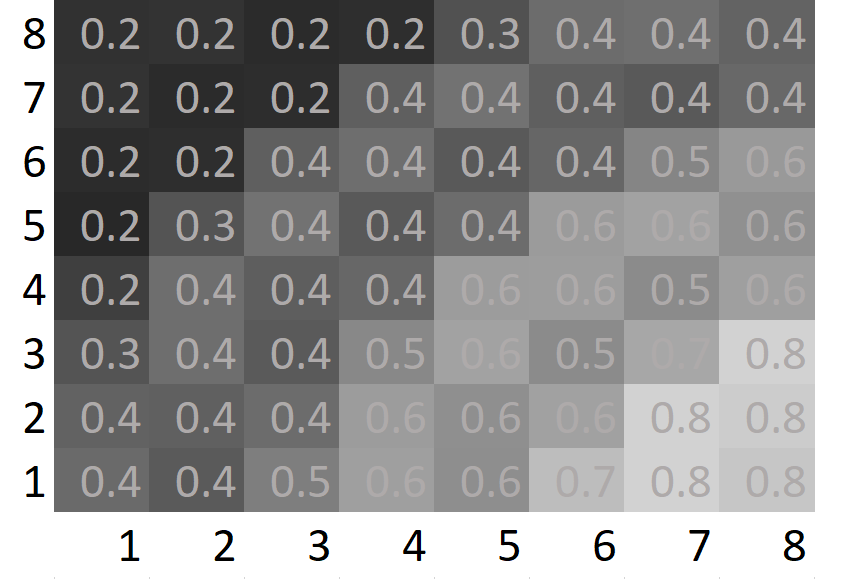
\includegraphics[width=0.45\linewidth]{image/grayscale-explain.png}
    \end{subfigure}
    \caption{ตัวอย่างภาพเฉดเทาที่แสดงระดับความเข้มของภาพในแต่ละระดับ}
    \label{figure:grayscale-explain}
\end{figure}

\hspace{1cm} จากภาพ \ref{figure:grayscale-explain} สังเกตว่าที่ค่าความเข้มของภาพเข้าใกล้ 0 จะให้สีเป็นลักษณะสีดำ ดังเช่นบริเวณที่พิกัดทางกายภาพเป็น (4,8) และเมื่อค่าความเข้มของสีเข้าใกล้ 1 จะให้สีที่มีลักษณะเป็นสีขาว ดังเช่นบริเวณที่มีพิกัดทางกายภาพเป็น (7,1)

\subsection{การต่อเติมภาพเฉดเทา}
\hspace{1cm} ในโครงงานวิจัยชิ้นนี้สำหรับการต่อเติมภาพ จะทำการหาคำตอบของภาพที่อยู่ในโดเมนต่อเติมภาพ ซึ่งจะของกำหนดตัวแปรต่างๆ ดังนี้

\hspace{1cm} ให้ $\Omega \subset \mathbb{R}^2$ แทนโดเมนภาพ (image domain) $D \subset \mathbb{R}^2$ แทนโดเมนต่อเติม (ดูรูปที่ \ref{figure:sample-domain}) และ $V \subset [0,\infty)$ และให้ $ u: \Omega \rightarrow V,\ z: \Omega \rightarrow V$ แทนภาพที่ได้รับการซ่อมแซมและภาพที่ต้องการซ่อมแซม ตามลำดับ

\begin{figure}[H]
	\centering
	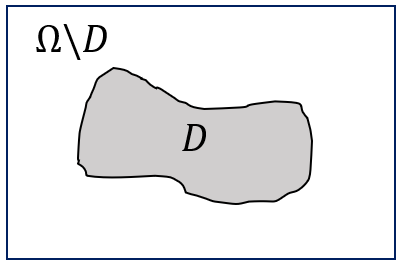
\includegraphics[width=0.375\linewidth]{image/sample-domain.png}
	\caption{$D$ แทนโดเมนต่อเติม}
	\label{figure:sample-domain}
\end{figure}

\hspace{1cm} การต่อเติมภาพเฉดเทาจะเป็นการหาคำตอบของพื้นที่ได้รับความเสียหายที่อยู่บนภาพ $z$ ซึ่งเป็นบริเวณในโดเมนต่อเติม $D$ โดยใช้ข้อมูลที่มีอยู่ใน $\Omega \textbackslash D$ เพื่อหาข้อมูลใน $D$ ที่ได้รับความเสียหายเป็นคำตอบในภาพ $u$

\subsection{การนำเสนอภาพสี}

\hspace{1cm} ต่อไปจะพิจารณาภาพสีในระบบ RGB นั่นคือ จะพิจารณาว่าภาพ $\boldsymbol{u}$ ประกอบด้วยสีด้วยกันทั้งสิ้น 3 คือ แดง, เขียว และ น้ำเงิน จึงเขียนภาพ $\boldsymbol{u}$  ในรูปแบบของเวคเตอร์ได้ดังนี้
\begin{align*}
	\boldsymbol{u} = (u_1,u_2,u_3)^{\top} : \Omega  \rightarrow V^3	
\end{align*}

\noindent เมื่อ $u_1,u_2,u_3: \Omega  \rightarrow V$ แทนภาพในเฉดสีแดง สีเขียว และสีน้ำเงินของ $\boldsymbol{u}$ ซึ่งการต่อเติมภาพสีที่พูดถึงในโครงงานวิจัยนี้จะทำการแยกแต่ละเฉดสีออกเป็นเฉดเทา 3 ระนาบ แล้วจึงใช้การต่อเติมภาพเฉดเทากับทั้ง 3 เฉดสีก่อนรวมกลับเป็นภาพสีอีกครั้ง
